%%
%% Copyright 2007, 2008, 2009 Elsevier Ltd
%%
%% This file is part of the 'Elsarticle Bundle'.
%% ---------------------------------------------
%%
%% It may be distributed under the conditions of the LaTeX Project Public
%% License, either version 1.2 of this license or (at your option) any
%% later version.  The latest version of this license is in
%%    http://www.latex-project.org/lppl.txt
%% and version 1.2 or later is part of all distributions of LaTeX
%% version 1999/12/01 or later.
%%
%% The list of all files belonging to the 'Elsarticle Bundle' is
%% given in the file `manifest.txt'.
%%

%% Template article for Elsevier's document class `elsarticle'
%% with numbered style bibliographic references
%% SP 2008/03/01
%%
%%
%%
%% $Id: elsarticle-template-num.tex 4 2009-10-24 08:22:58Z rishi $
%%
%%
\documentclass[preprint,12pt,3p]{elsarticle}

%% Use the option review to obtain double line spacing
%% \documentclass[preprint,review,12pt]{elsarticle}

%% Use the options 1p,twocolumn; 3p; 3p,twocolumn; 5p; or 5p,twocolumn
%% for a journal layout:
%% \documentclass[final,1p,times]{elsarticle}
%% \documentclass[final,1p,times,twocolumn]{elsarticle}
%% \documentclass[final,3p,times]{elsarticle}
%% \documentclass[final,3p,times,twocolumn]{elsarticle}
%% \documentclass[final,5p,times]{elsarticle}
%% \documentclass[final,5p,times,twocolumn]{elsarticle}

%% if you use PostScript figures in your article
%% use the graphics package for simple commands
%% \usepackage{graphics}
%% or use the graphicx package for more complicated commands
%% \usepackage{graphicx}
%% or use the epsfig package if you prefer to use the old commands
%% \usepackage{epsfig}

%% The amssymb package provides various useful mathematical symbols
\usepackage{amssymb}
%% The amsthm package provides extended theorem environments
%% \usepackage{amsthm}

%% The lineno packages adds line numbers. Start line numbering with
%% \begin{linenumbers}, end it with \end{linenumbers}. Or switch it on
%% for the whole article with \linenumbers after \end{frontmatter}.
\usepackage{lineno}

%% natbib.sty is loaded by default. However, natbib options can be
%% provided with \biboptions{...} command. Following options are
%% valid:

%%   round  -  round parentheses are used (default)
%%   square -  square brackets are used   [option]
%%   curly  -  curly braces are used      {option}
%%   angle  -  angle brackets are used    <option>
%%   semicolon  -  multiple citations separated by semi-colon
%%   colon  - same as semicolon, an earlier confusion
%%   comma  -  separated by comma
%%   numbers-  selects numerical citations
%%   super  -  numerical citations as superscripts
%%   sort   -  sorts multiple citations according to order in ref. list
%%   sort&compress   -  like sort, but also compresses numerical citations
%%   compress - compresses without sorting
%%
%% \biboptions{comma,round}

% \biboptions{}

%Todd added this for strikeout \sout{}
\usepackage[normalem]{ulem}
%Todd added this for the reference to essence.sv.cmu.edu
\usepackage{hyperref}


\journal{Todd Sedano's ECE Prospectus Committee}

\begin{document}

\begin{frontmatter}

\title{Adopting Essence Kernel, Understanding Agile Iterative Software Development}

\author{Todd Sedano}
\ead{professor@gmail.com}

\author{C\'ecile P\'eraire}
\ead{cecile.peraire@sv.cmu.edu}

\address{Carnegie Mellon University}
\address{Silicon Valley Campus}
\address{Moffett Field, CA 94035, USA}


\begin{abstract}
Software development continues to be a complex endeavor involving many disciplines and skill sets. Practitioners and researchers continue to experiment, research, and adopt practices to simplify, understand, and create repeatable processes. 

The Software Engineering Method and Theory (SEMAT) community created the Essence kernel as a unifying framework for describing and analyzing software engineering endeavors. The framework consists of an Essence kernel containing ``universal" project dimensions, states, and checkpoints found on every software engineering project. Practices such as ``Code Review" or ``Pair Programming" specific to certain circumstances are built on top of the kernel. Software methods compose these practices into logical groupings. The SEMAT community claims that Essence helps practioners by providing a rigous foundation and understanding to all software endeavors. 

At Carnegie Mellon University in Silicon Valley, I conducted a field study with masters of science in software engineering students as they completed a team-based capstone project course using the Essence kernel. During the weekly Essence Reflection meetings, the Essence kernel provided goals for the students to achieve. The student teams found value during project inception, start-up, and project wrap-up. The teams found little value during an iterative construction phase as the Essence kernel offered no new goals. The original Essence kernel is method agnostic and does not directly support iterative development. Since most of agile software development occurs via iterative software development, adapting Essence kernel to have would goals during iterative construction phase would increase its value to software development teams.

My next goal is to adapt the Essence kernel for use at Pivotal by providing a kernel extension to match Pivotal's engineering practices. My plan is to conduct participant-observation of several software development projects at Pivotal. I will interview many software engineers and product managers to collect additional data. I'll iterative my research by incorporating this feedback. For validation, I will review the proposed Pivotal Extension with software engineers and product managers. My expected results is a modified kernel or kernel extension grounded in empirical data that supports iterative software development. 

\sout{I have demonstrated that generic algorithms can be used to create kernels from empirical data. I created the Partial Ordering fitness function for evaluating candidate kernels against empirical data. The research shows that alternative structures for the kernel are necessary to best reflect the data.}

\sout{I created a research tool.}
\end{abstract}

\begin{keyword}
%% keywords here, in the form: keyword \sep keyword
Essence Kernel \sep Empirical Research \sep Iterative Software Development
%% MSC codes here, in the form: \MSC code \sep code
%% or \MSC[2008] code \sep code (2000 is the default)
\end{keyword}

\end{frontmatter}

%%
%% Start line numbering here if you want
%%
%%\linenumbers

\section{Introduction}

\subsection{Problem Statement}
Software engineers can struggle with effectively running software projects. Researchers and practitioners have examined ways to handle the ``software crisis" since as early as the first Nato Software Engineering Conference in 1968 \cite{Naur1969}. The SEMAT community created Essence (described in more detail in Section \ref{Method}) as a universal framework for any software engineering project.  Software development teams can use Essence Reflection meetings \cite{EASE2014} to track and monitor their progress throughout a software project. 

\subsection{Research Objective}
\sout{Update this section}

Following recommendations for reporting research done in the empirical
software engineering community
\cite{GQM, Shaw}, I formed the
research goal using Goal/Question/Metric:
\cite{GQM}

\begin{table}[h]
\centering
\begin{tabular}{|p{2.00in}|p{4.10in}|}
\hline
Analyze & kernel extensions for iterartive software development \\ \hline
for the purpose of & evaluation \\ \hline
with respect to its & effectiveness \\ \hline
from the point of view of the & software engineer and researcher \\ \hline
in the context of & software development at Pivotal. \\
\hline
\end{tabular}
\end{table}

\subsection{Method under Investigation}
\label{Method}

The SEMAT community created Essence as a universal framework for any software engineering project. At the core of Essence is a ``kernel of widely-agreed elements'' ~\cite{JacobsonQueue}. This general kernel can theoretically support any kind of software endeavor. A software project can define its software processes by using the general kernel, extending the kernel, or defining additional practices on top of the kernel.

\begin{figure}[h]\vspace*{4pt}
\centerline{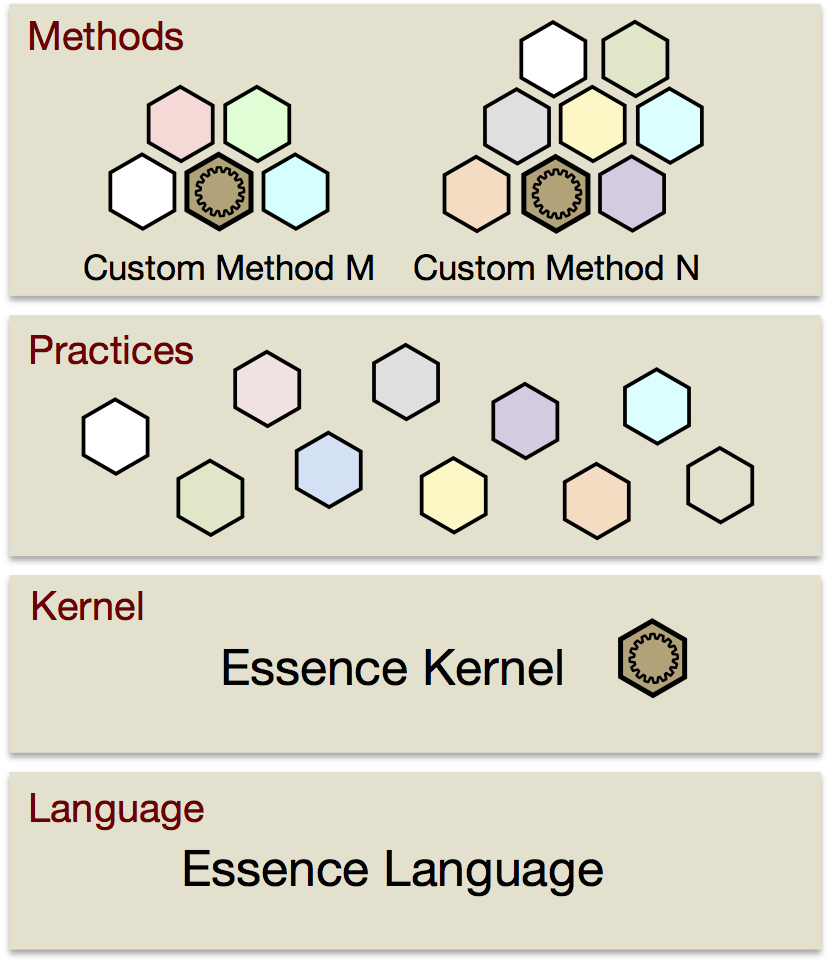
\includegraphics[width=2.2in]{kernel_images/EssenceLayers}}
\caption{Essence Method Architecture: Methods and Practices are Context Specific and the Kernel is Universal}\vspace*{-6pt}\label{EssenceLayers}
\end{figure}

The Essence kernel is composed of a set of alphas, alpha states, and alpha state checkpoint items. The Essence kernel defines different characteristics or dimensions of a software project as an ``alpha.'' The seven alphas are \textbf{Stakeholders}, \textbf{Opportunity}, \textbf{Requirements}, \textbf{Software System}, \textbf{Team}, \textbf{Way of Working}, and \textbf{Work}. Essence decomposes each of these alphas into a set of states that represent a simple linear state machine as shown in Figure \ref{StateMachine}. For example, the \textbf{Requirements} alpha advances through the states \textit{Conceived}, \textit{Bounded}, \textit{Coherent}, \textit{Acceptable}, \textit{Addressed}, and \textit{Fulfilled.} Each state has a checkpoint or set of goals. To achieve a state, the project must satisfy every checkpoint item for that state. \cite{OMGStandard} 
 
\begin{figure}[h]\vspace*{4pt}
\centerline{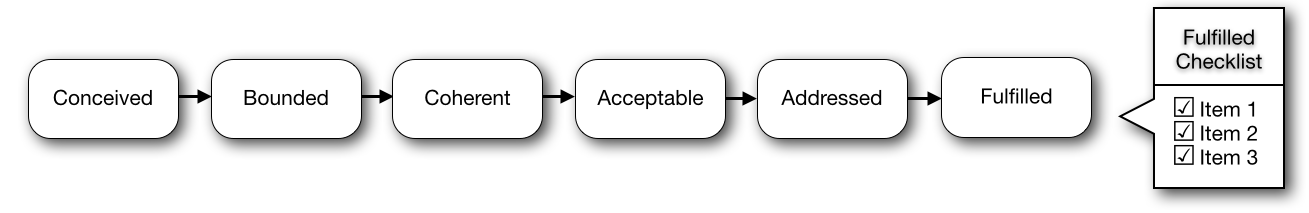
\includegraphics[width=5.4in]{kernel_images/StateMachineRequirements}}
\caption{Kernel's linear state machine for Requirements alpha (with Fulfilled checkpoint)}\vspace*{-6pt}\label{StateMachine}
\end{figure}

\subsection{Prospectus Outline}

Sections \ref{EssenceReflectionMeetings} through \ref{KernelOptimization} summarize my research to date. My referenced published papers provide additional detail. Because I value the committee's input and feedback on the final portion of my research, a significant portion of this prospectus focuses on Section \ref{PivotalKernelExtension} . 

In Section \ref{EssenceReflectionMeetings}, I will define Essence Reflection meetings where a facilitator guides a team through the Essence kernel for the purpose of project monitoring and steering. This work was presented at EASE 2014 \cite{EASE2014}.

In Section \ref{CMUFieldStudy}, I summarize a field study's results showing the value in applying Essence Reflection meetings in graduate software engineering program at Carnegie Mellon University in Silicon Valley. This work was presented at ICSE 2014 \cite{ICSE2014}. The field study revealed that the kernel does not reflect incremental progress achieved during construction on iterative projects. Section \ref{PivotalKernelExtension} describes my research plan on addressing this issue.

In Section \ref{EssenceTool}, I describe a web-based tool that I wrote to facilitate data-collection, simplify the introduction of Essence Alphas during Essence Reflection meetings, and aid in analyzing the collected data. The tool is available at \url{http:\\esssence.sv.cmu.edu}

In Section \ref{KernelOptimization}, I summarize my work in using genetic algorithms to create random kernels based on empirical data, unlike the original kernel which is based on human experience and judgment. My research shows that kernels with smaller number of alphas result in higher fitness scores than the original kernel. Based on the analysis of the fitness function, a kernel with a fundamentally different structure might more effectively recommend next steps for a team during Essence Reflection meetings. I presented this work at SCSE 2015.

In Section \ref{PivotalKernelExtension}, I outline my research plan for a kernel extension or kernel replacement that supports iterative software development projects. I will use empirical data collected from field observations, participant-observation, and interviews to derive an iterative kernel. 


\section{Essence Reflection Meetings}
\label{EssenceReflectionMeetings}

The EASE 2014 paper presents an empirical evaluation of the team reflection support provided by the Essence framework, and compares Essence reflection meetings to other types of team reflection meetings.

Essence Reflection meetings are an alternative to Agile retrospection or weekly status meetings. 

During an Essence Reflection meeting, a team systematically uses the Essence kernel to identify where they are in the project, identity next possible goals, and generate action items to achieve those goals. 

For each alpha, team members ...
\begin{enumerate}
\item Read Alpha State Checklists
\item Identify Current State
    \begin{itemize}
    \item Individually and silently determine the current state
    \item When ready, all reveal their state at same time.
    \item Discuss differences of opinion until agreement is reached.
    \item Record current state
    \end{itemize}
\item Perform Root Cause Analysis
    \begin{itemize}
    \item Discuss why the target state is not achieved.
    \end{itemize}
\item Determine Action Items    
\end{enumerate}

The team members step back from their daily tasks, come together as a team, and look 
at the project holistically based on the seven alphas.

The team monitors its progress by identifying the current state of each alpha. 

The team sets the project direction by identifying the target state for each alpha. Following a discussion focusing on why a target state is not achieved, the team sets the goals to reach that state. The goals are selected out of the target state checklist.

The team decides how to reach the goals associated to each target state by defining some specific work items. The kernel does not.

The identified work items have been added to the team’s work item list or backlog. The team members return to their office space and start working on the work item. 

After awhile (typically a week in our case), the team regroups again, and looks at the project holistically based on the seven project dimensions. This is an iterative process allowing the team to monitor and steer the project towards higher states.

I created Essence Reflection meeting as pragmatic re-framing of an idea found in Chapter 8 of \underline{The Essence of Software Engineering} \cite{EssenceBook}. The original idea suggested that a team meeting meet at the beginning of an iteration, identity which state cards to achieve at the end of the iteration, and identity tasks to put in the backlog. Instead, in my approach, there is no expectation that any state would be accomplished by the end of an iteration. Goals are identified to achieve in the future. Action items generated in this meeting might not be appropriate for a software development backlog, and thus are treated separately from tasks. I further refine the activity to have explicit root cause analysis steps. 

\section{Kernel Evaluation in Academic Graduate Programs}
\label{CMUFieldStudy}
I performed a field study \cite{ICSE2014} that showed that Essence Reflection meetings \cite{EASE2014} using the Essence kernel provide project teams with a simple, lightweight, non-prescriptive and method-agnostic way to examine their projects holistically, structure team reflections, manage risks, monitor progress and steer their projects. The purpose of the field study was to to understand the value project teams receive from following the SEMAT Essence’s monitoring and steering approach provided by the Essence kernel alphas and their states. The two semester field study followed seven master of software engineering teams with no prior knowledge of Essence in a team-based capstone course called, ``Software Engineering Practicum." Compared to the ten previous years, the faculty in charge of the practicum course noted that there was ``much better early project organization with a lot less floundering." Indeed, the approach enabled students to learn to steer projects effectively by addressing the various dimensions of software engineering.

The field study showed that most of the value from the Essence kernel occurs during project startup and initiation and for monitoring and steering the work done at the project or release level \cite{ICSE2014}. Since the work is done at the project or release level, it could be qualified as ``universal" as it is generally common across projects. This confirms that the kernel provides an effective support for universal work. Support for non-universal technical work should come from additional practices added on top of the kernel, or by extending or altering the kernel definition.

\section{Kernel Support and Tooling}
\label{EssenceTool}
I created a research tool for supporting team-based software development for the purpose of increasing the efficiency of Essence Reflection Meetings, decreasing training time, and streamlining data collection. A screen-shot of the tool is shown in Figure \ref{EssenceToolScreenshot}. Before the tool existed, I would print out the alphas and using a paper cutter, cut out each individual state card for each alpha. This was time consuming and laborious. Transporting and handing out a set of cards to each team member was tedious as I had to be careful not to mix them up. (insert photo) In the next semester, I printed out a full strip of alpha cards on legal paper. See Figure \ref{AlphaStrip}, cutting continued to be time consuming. For distributed teams we used google documents' diagrams, but it was slow and tedious to zoom in and zoom out (insert picture). For data entry we used google spreadsheets to capture which checklists the students achieved each week. Once the semester was over we would convert this data into different representations to create graphs to show team progress through the semester and to help us analyze the data.  

\begin{figure}[ht]
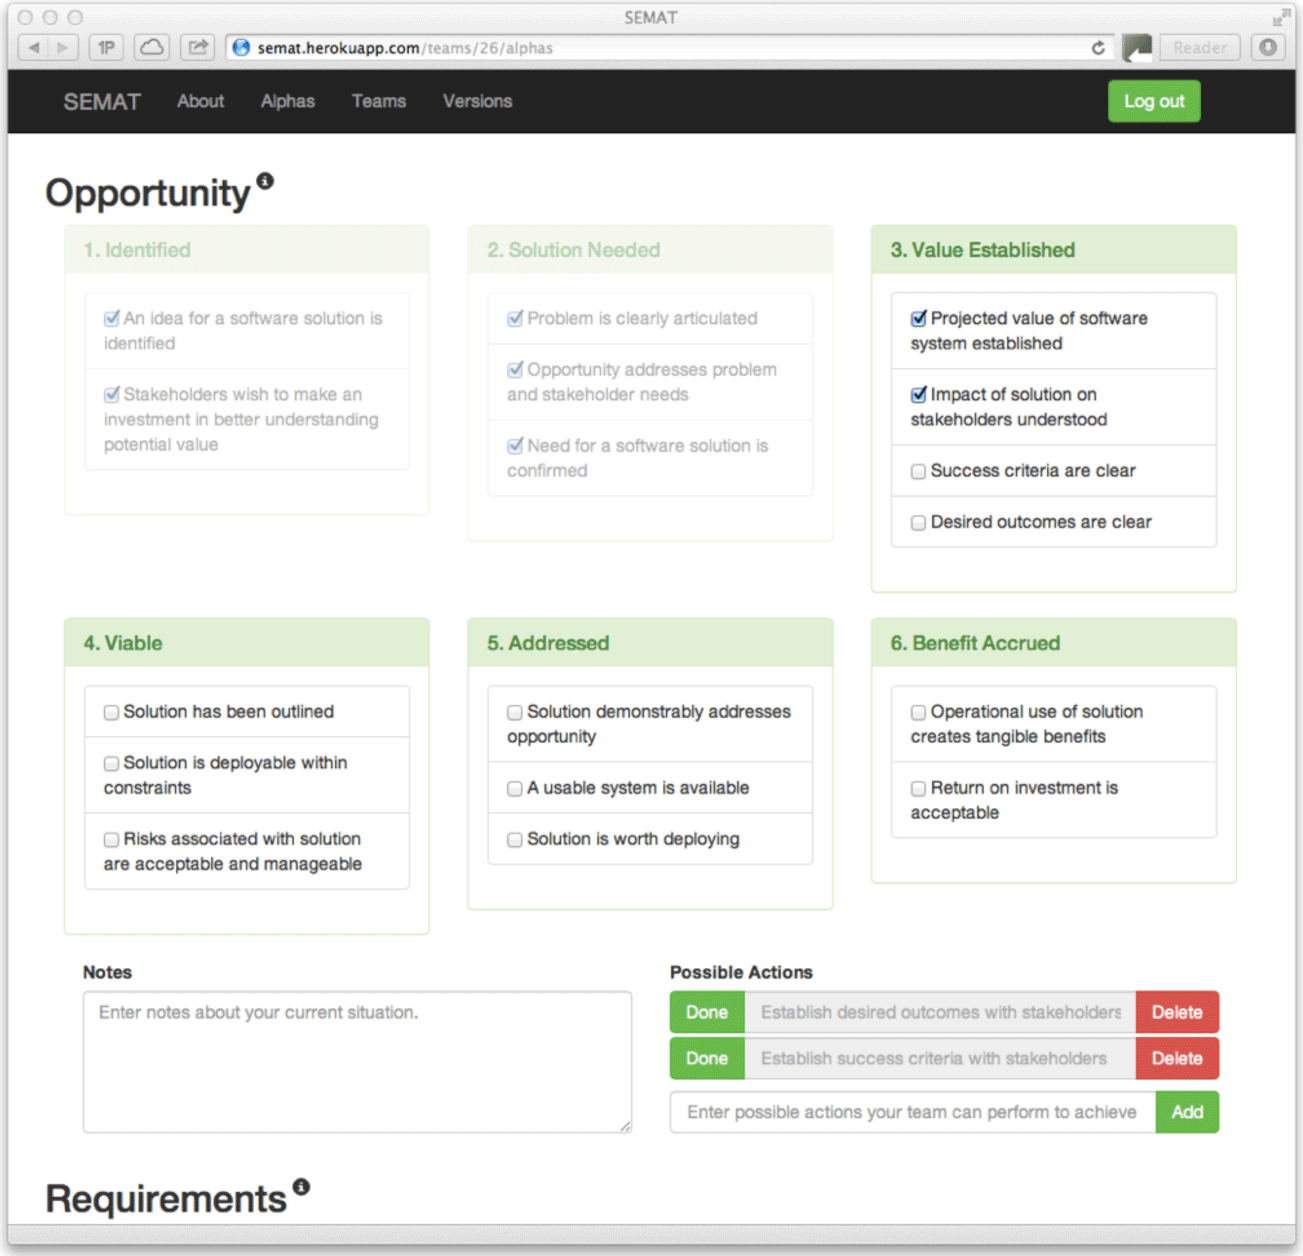
\includegraphics[width=6.15in]{tool_photos/tool_photo}
\caption{Essence Kernel Tool for Essence Reflection Meetings}
\label{EssenceToolScreenshot}
\end{figure}

\begin{figure}[ht]
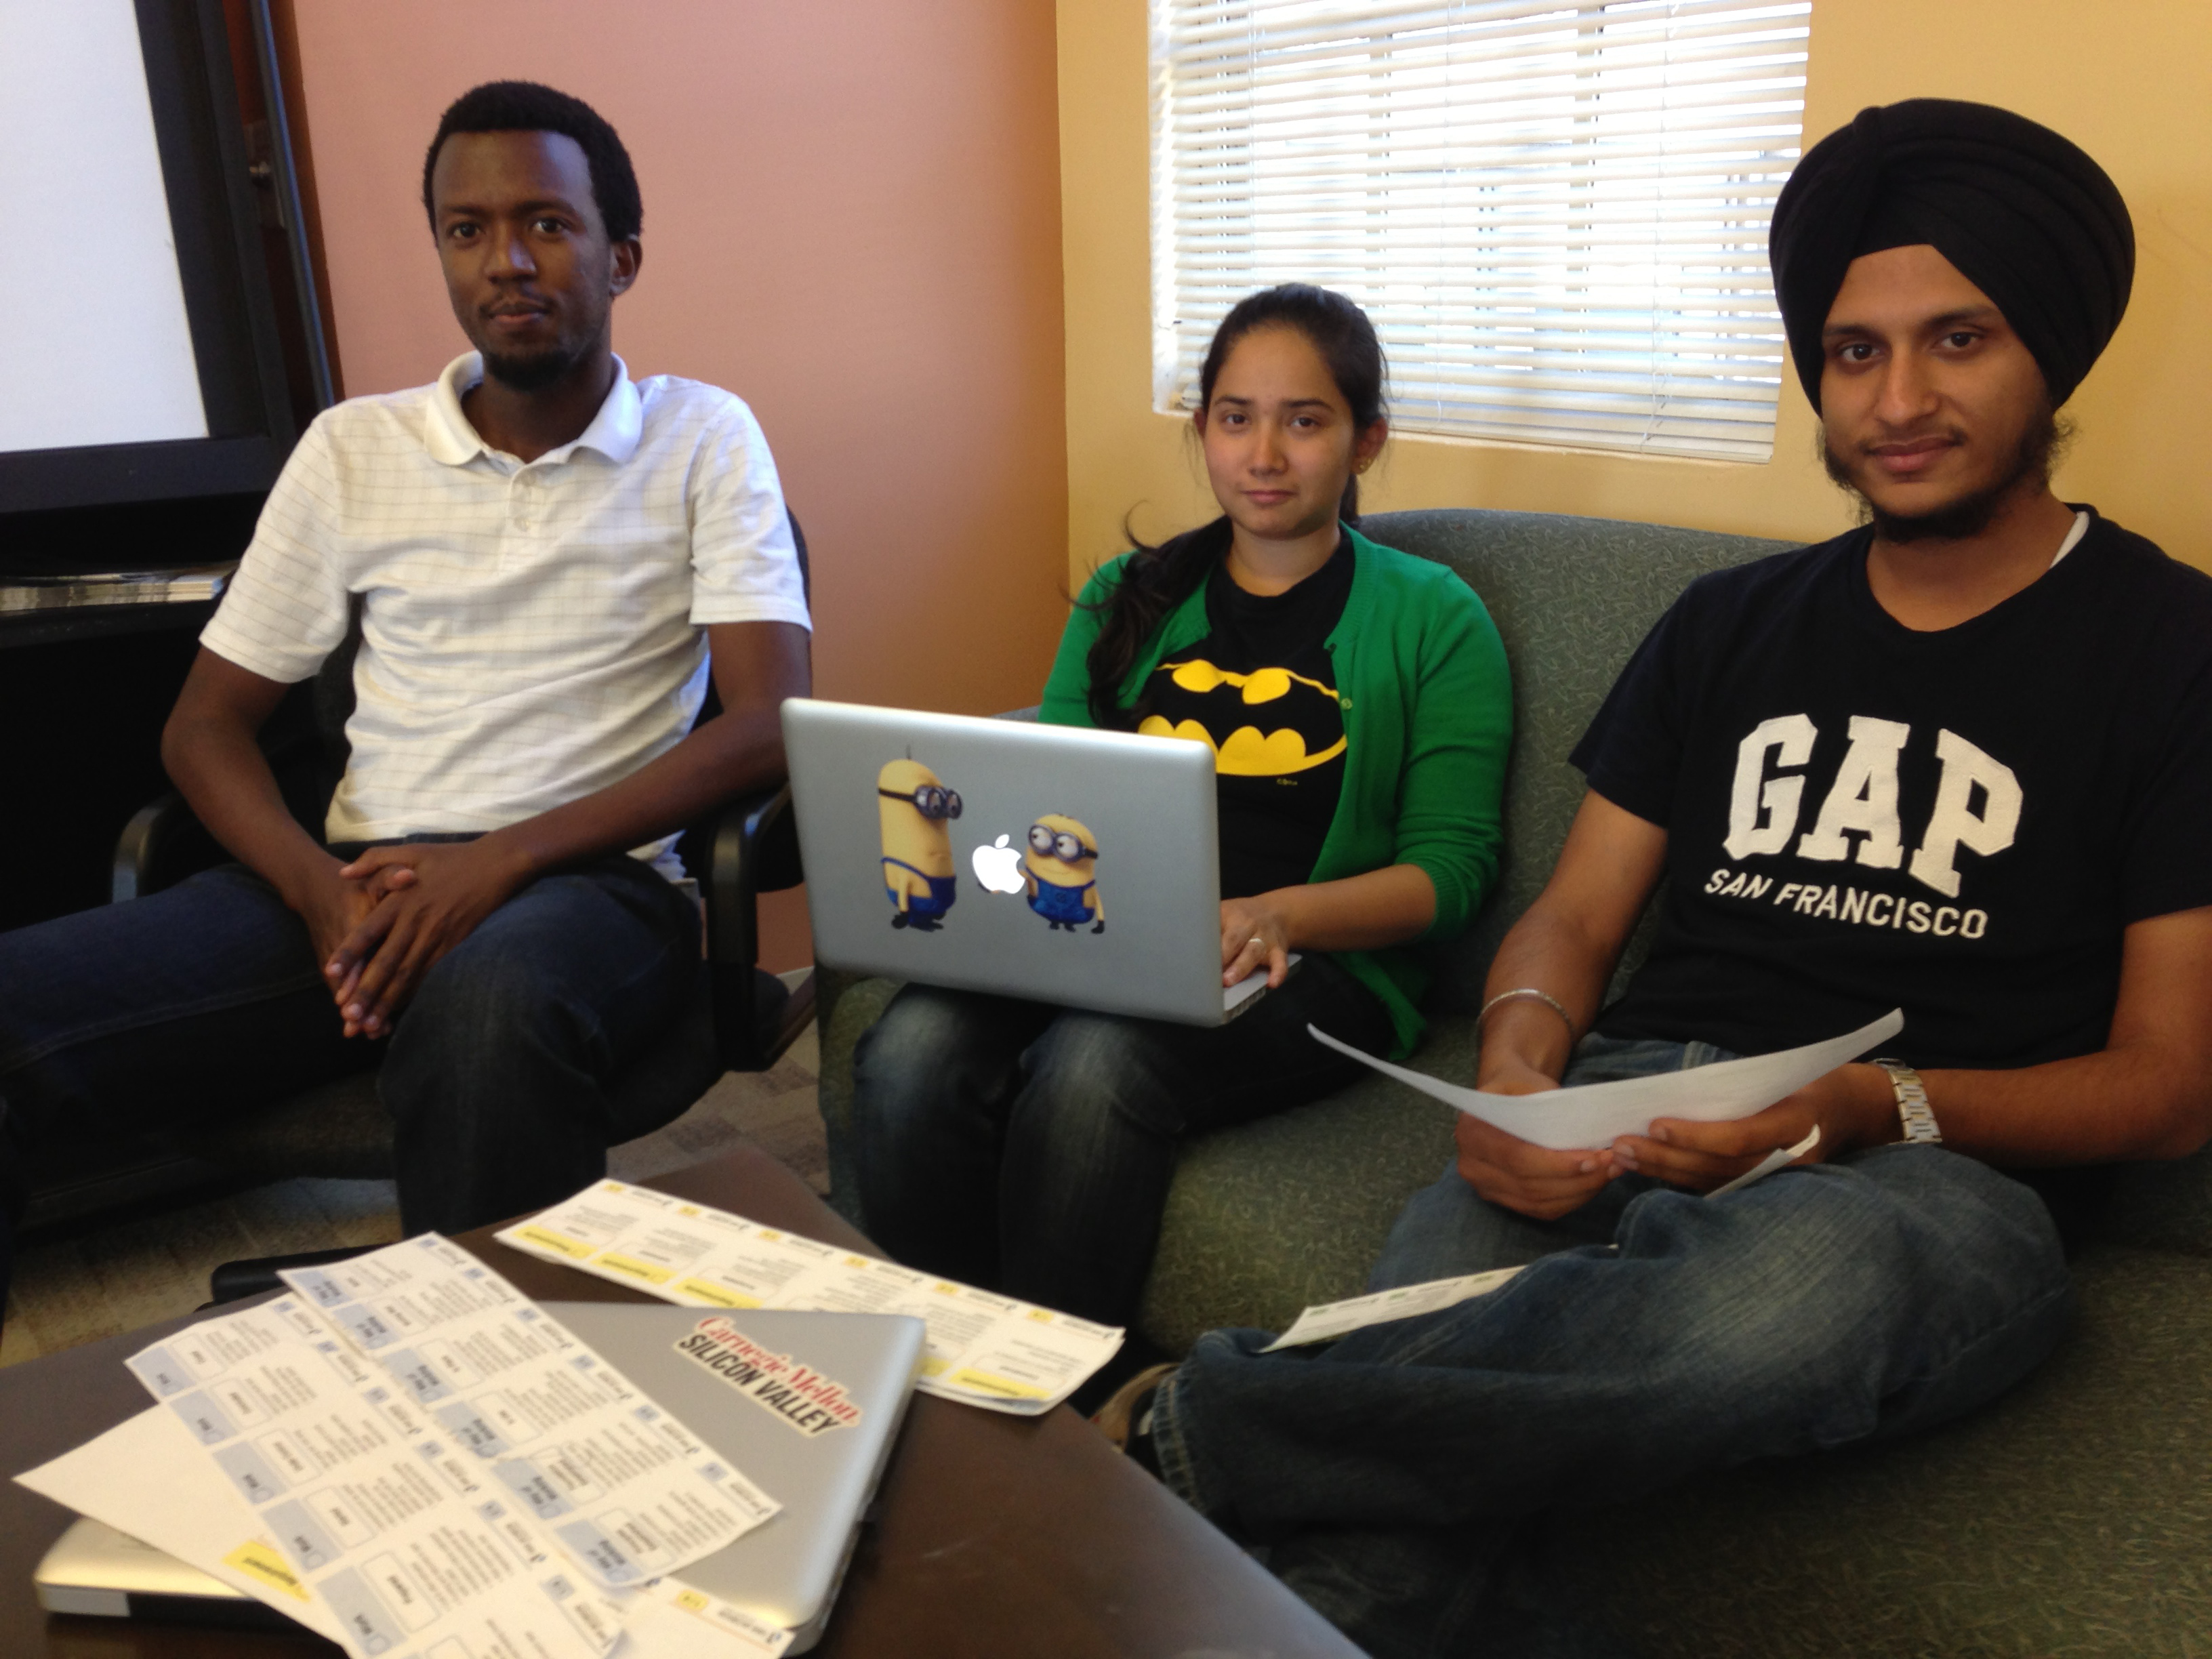
\includegraphics[width=6.15in]{student_photos/team_1}
\caption{Student Team using an Alpha Strip during an Essence Reflection Meeting}
\label{AlphaStrip}
\end{figure}

The tool enabled us to streamline the entire process. Prior to the first Essence Reflection meeting, a faculty member log ins in, creates a team, and adds each student member to the team. During the first meeting, one team member shows the first alpha on a projector or TV screen in a conference room. The tool helps the team focus on the kernel, one alpha at a time. Before the data was presented on a sheet of paper and the data was collected in a spreadsheet; now the tool allows kernel viewing and data collection to happen at the same place. Once the team is done entering their information, the "done" button emails everyone on the team including the faculty member the team's current status for each alpha, all captured notes, and a list of action items for the team to accomplish. 

I conducted usability testing on the tool and incorporated the feedback into the tool. This enabled me to improve the tool's usefulness and reduce issues for novice users. 

\section{Kernel Optimization}
\label{KernelOptimization}
After creating a research and educational tool described in Section \ref{EssenceTool}, I collected empirical data on how teams progress through the Essence kernel during their project. I leveraged genetic algorithms to generate candidate replacement kernels by using a fitness function based on empirical data. When the SEMAT community created the Essence kernel, they relied upon human experience and judgment to select the alphas, states, and checklists. Essence is not grounded by empirical data. The generated kernels outscored the original. The purpose of that exploratory work was to demonstrate one way to generate a candidate Essence kernel directly from empirical data, not to recommend a replacement for the original Essence kernel. \cite{SCSE2015}

While the original kernel appears to be descriptive and the kernel does claim to support any software project, in practice, the kernel is a prescriptive representation. First, the kernel is based on expert experience not directly from project data. Second, when discussing potential modifications to the original kernel based on my project data, the kernel committee (what's the official name?) made comments to the effect of ``that's a nice suggestion, but we don't think that would generalize to all projects" and ``that's a nice suggestion, but I want to represent how projects should be run, not how they are actually run." 

\section{Kernel Extension in Industry}
\label{PivotalKernelExtension}
Because the Essence kernel is software methodology agnostic, it does not directly provide support for iterative software projects \cite{ICSE2014} and relies on kernel extensions. Students following Scrum did not find following the kernel extension for Scrum to be helpful. Students successfully followed Scrum without any support from the Essence framework.

Pivotal has followed Extreme Programming \cite{ExtremeProgrammingExplained} since the late 1990's. Pivotal Labs transforms their client's engineering cultures into agile ones by augmenting the client's software engineers with Pivotal's engineers to deliver a software product. For start-ups, Pivotal might be the first engineers working on the project. For enterprise clients, Pivotal provides additional engineering resources to accomplish new business goals or Pivotal helps transform engineering cultures when they no longer routinely deliver code.  While each team is autonomous in making its own decisions as to what is best for a particular project, the company culture strongly suggests following all of the core practices of Extreme Programming including Pair Programming, Test Driven Development, Weekly Retrospections, Daily Stand-ups, Prioritized Backlog, Whole Team ownership of the project and code base, and Kanban's notion of work flowing through people. 

With a stable and consistent way of working, Pivotal provides an research opportunity to demonstrate how a kernel modification or extension could support iterative software development. 

The Essence kernel is based upon human experience and judgment, not empirical data. Th goal is to derive a kernel extension for iterative software projects directly from empirical data. 

Research Question 1: Does the kernel support software development as it is done at Pivotal? (Is it what you do at pivotal in satisfy what is in the kernel, does the kernel describe what is happening at a high level.)

Research Question 2: Is Essence useful? Why are you not using it? Is it helping at pivotal? 

Research Question 3a) How would you modify the kernel? 

Research Question 3b) How would you extend the kernel to incorporate iterative development as it is done at Pivotal?

Research Question 4: How does the extension compare to other Essence components such as the Requirements-Item Sub-Alpha and the Software-System Alpha? 

Research Question 5: How does it compare to Scrum?

\subsection{Context}
Pivotal provides solutions for cloud-based computing, big data, and agile development. Pivotal Cloud Foundry is an open source Platform as a Service for on-premise or hosted in the cloud. Pivotal Big Data Suite stores and analyzes multiple large data sets using Hadoop, Hawq, and Green Plum. Pivotal Labs provides agile developers and designers for start ups and enterprise companies. Pivotal Labs has offices in San Francisco, Palo Alto, Los Angeles, Boulder, Denver, Chicago, Washington District of Columbia, Toronto, and London.  

The methodology under study is Extreme Programming. \cite{ExtremeProgrammingExplained} Pivotal Labs has used Extreme Programming since the late 1990s to enable collaborative experiences for Pivotal Labs clients.

For this study, the experience of the participants will range from 0 to 20 years of experience in industry. I will select participants with at least six months of experience at Pivotal Labs. The size of the projects will range from 4 to 30 engineers.

Pivotal created Pivotal Tracker for supporting its software development workflow by capturing key information from product managers, sharing that information with software engineers, and yielding project monitoring for any interested party. Eventually, Pivotal releases Pivotal Tracker for any software company following agile software development.

Section \ref{FieldStudyPlanning} \textit{Field Study Planning}, describes the research plan, procedure, and participant selection. Section. \ref{ExpectedResults} \textit{Expected Results}, provides an kernel extension example. Section \ref{Discussion} \textit{Example Discussion}, discusses the results. 
%Section. \ref{Conclusions} presents conclusions and future work.

\subsection{Description of Related Studies}

\textbf{I'm currently planning to comment out this section.}

Elves{\ae}ter et al \cite{Elvesaeter2013} describe a kernel extension for the agile method Scrum \cite{Schwaber2001} for the purpose of comparing and contrasting Essence with Software \& Systems Process Engineering Metamodel (SPEM) 2.0. The Scrum Guides \cite{ScrumGuide} served as a source definition for Scrum. 
 In the example, they break down the work at the Sprint or iteration level. The \textbf{Sprint} sub-alpha extends the \textbf{Work} alpha and has the states \textit{Planned}, \textit{Started}, \textit{Under Control}, \textit{Concluded}, and \textit{Closed}. Each state is defined with its own checkpoint items. 

Since the \textbf{Sprint}'s checkpoints are independent of the \textbf{Work}'s checkpoints, a team could progress through one, several, and even every Sprint without achieving all of the Work checkpoint items. For example, the work might never be fully ``broken down into actionable work items with clear definitions of done" until the end of the project. Likewise many agile methods strongly discouraging re-estimating work \cite{} where as the \textbf{Work} alpha includes the required ``estimates are revised to reflect the team’s performance" checkpoint. 

The work relies on \textbf{Tasks} in the Task Management Extension defined in the OMG Proposal \cite{OMGStandard}. \textbf{Tasks} are the work items to be accomplished during a \textbf{Sprint} that are prioritized in the Product Backlog activity. The \textbf{Task} alpha supports the \textbf{Work} alpha and has three states \textit{Identified}, \textit{In Progress}, and \textit{Done} as described in Figure \ref{TaskDefinition}

\begin{figure}[h]\vspace*{4pt}
\caption{Task Definition}\vspace*{-6pt}\label{TaskDefinition}
\textit{Identified} - The task has been identified and is ready to be done.
\begin{itemize}
\item A portion of work has been clearly identified and isolated.
\item The objective of the Task is clear.
\item The things that need to be done have been clearly described.
\item It is clear whether the task is a whole team task, group task or individual task.
\item The completion criteria for the task are clearly defined.
\item The effort required to complete the task has been estimated and agreed.
\end{itemize}

\textit{In Progress} - The task has been accepted by one or more team members and work has started.
\begin{itemize}
\item A team member has accepted and is progressing the task.
\item The progress of the task is monitored.
\item A target completion date for the Task has been agreed. 
\item The amount of effort required to complete the task is being tracked.
\end{itemize}

\textit{Done} - The work required to do the task has been completed.
\begin{itemize}
\item Work on the Task has stopped.
\item The task is determined to be complete according to its completion criteria. 
\end{itemize}
\end{figure}

The definition of the \textbf{Task} alpha is based on human experience and judgement. From Pivotal's perspective, there are issues with this description. Pivotal has no need to track the actual effort of a story. This means that \textit{In Progress} would never be achieved since the fourth checkpoint is never reached. Work on a story can stop and has no correlation witha task being done, in contrast to the first checkpoint of \textit{Done}. 

\subsection{Field Study Planning} 
\label{FieldStudyPlanning}

\subsubsection{Goals}
The goal is to generate a kernel extension or replacement kernel that models the practices used by product managers and software engineers at Pivotal to manage their projects.

\subsubsection{Generating the initial kernel extension}
I followed the participant-observer technique by joining a software development team as a full time software engineer. I contributed as an equal member of the team by writing code and attending all team meetings for 40 hours per week. 

As software development occurred, I would reflect on the software development experience and record notes. After examining my notes I created a representation model to explain the observations. I would continue to collect data and update the model when the model did not fully describe the data. I would periodically review the kernel extension for missing elements. Empirical data collected across multiple projects and interviews forms the foundation for the proposed kernel extension. Figure \ref{KernelExtensionWorkflow} and Figure \ref{KernelExtension} illustrate the current proposal.

When special circumstances arose during a project, I would collect additional data. For example, during one project, the product manager rejected a large number of stories. I reviewed each rejected story to ascertain the reason why the product manager rejected. I then modified the model to incorporate this information.

\subsubsection{Validating the kernel extension}

In order to refine and validate the kernel extension, I plan to interview Pivotal product managers and Pivotal software engineers. Even though the two roles have different perspectives, I'll use the same interview questions because I'm after one goal, a model that describes the way Pivotal does iterative software development.

I plan to use semi-structured interviews. This allows me to ask the same questions of every interview candidate, but also explore and follow-up on interesting perspectives of a participant. \sout{There is a publishing risk as I believe reviewers focus on the printed questions that are asked in every interview.}

\begin{itemize}
\item Please describe your typical day? What is the day in the life of a product manager / software engineer?
\item What are the characteristics and attributes on an ideal story?
\item What is the purpose of the iteration planning meeting?
\item How can you tell if a story is ready for iteration planning meeting and thus ready to be pointed?
\item What feedback go you get that the project is working well?
\item Where does usability testing fit into your ideal project?
\item Please describe your workflow by drawing it on this blank piece of paper.
\item Please examine this proposed model and critique it.
\end{itemize}

I will record and transcribe these conversations. I will annotate the transcription with markers and use these to update the proposed model.

Based on one trial run of these questions, I expect the conversations to last between thirty and forty minutes. 

I have some open questions
\begin{itemize}
\item Do I interview all the product managers then software engineers? or do I co-mingle the interviews?
\item What ratio of product managers to software engineers.
\end{itemize}

I would like to skip the first question for software engineers.

\sout{Finally, software engineers will be shown the proposed kernel extension. Participants will asked to reflect on their experience at following Extreme Programming at Pivotal and then respond to the proposed kernel extension.}

\subsection{Participants}
For the participant-observer portion of the research, I %the embedded participant researcher 
observed three sequential projects.  I selected these projects for study opportunistically based upon my allocation to projects.

Project one had 210 stories. The project was a web front end for a cluster server using Angular and Ruby on Rails. The project lasted 13 weeks and I worked with and observed the team for the last seven weeks of the project. 

Project two had 387 stories. The project was an e-commerce tool for a publishing company. The project lasted 19 weeks and I worked with and observed the team the entire time.

Project three had 267 stories. The project was a web administrator tool for internet service providers. The project lasted eight weeks I worked with and observed the entire project.

Since I'm in a new and growing office, I plan to be opportunistic in my interviewing. I plan to interview our most experienced product manager recently left Pivotal and joined a start up. Our only office product manager is new to Pivotal, and I plan to interview him last. I plan to travel to the San Francisco office to interview product managers there. I plan to interview client product managers although their perspective may not be congruent with Pivotal's way of working. If the model hasn't reached saturation, I plan to interview product managers from one of Pivotal's nine international offices.

For software engineers, I plan to interview software engineers at Pivotal who worked on projects at the Silicon Valley office. I will choose the participants so that I have a broad representation of the office. Their professional experience will probably range from two to 20 years of experience. 

Participants will not be paid for their time. 

\subsection{Expected Results}
\label{ExpectedResults}

I expect to be able to derive a kernel extension representing Pivotal's approach to iterative software development based upon the  observations and collected data from the previous section.

As an example of the expected results, I include here my initial results of the \textbf{Story Card} alpha from observing several projects. Section \ref{Discussion} discusses Figure \ref{KernelExtensionWorkflow} and Figure \ref{KernelExtension} in detai.

Since Pivotal follows Extreme Programming, there's a risk that the results will simply reproduce what is already known about Extreme Programming. (Currently to our knowledge, no one has shown how to model Extreme Programming with Essence.) The provided checkpoints are unique to this research and are not included in Extreme Programming. I would expect that the results could be applicable to other teams that follow Extreme Programming. 

So far, the initial results are modeling the process practices of Extreme Programming, not the technical practices such as Pair Programming and Test Driven Development. Since Extreme Programming is mostly Scrum plus a set of technical practices, this means that the model could be useful to Scrum projects. This also means that the results can be compared to the previous Scrum kernel extension.

Again, these are initial, representative results which could change dramatically as I collect more data and refine the model.

\begin{figure*}[ht]
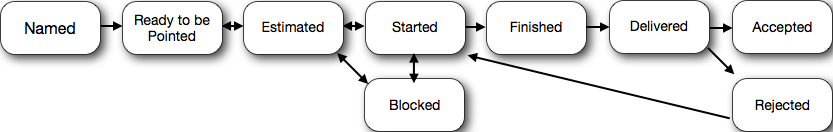
\includegraphics[width=6.25in]{pivotal_images/story_card_workflow}
\caption{(Initial Results) Pivotal Kernel Extension Workflow Story Card Alpha}
\label{KernelExtensionWorkflow}
\end{figure*}

\begin{figure*}[ht]
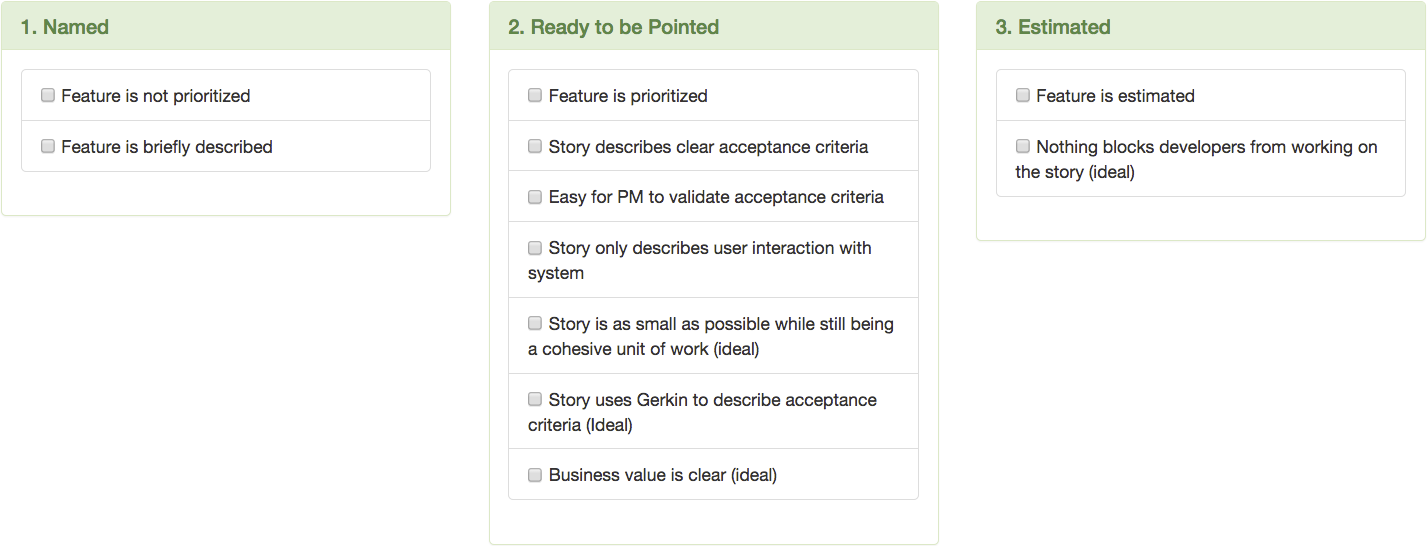
\includegraphics[width=6.25in]{pivotal_images/story_card1}
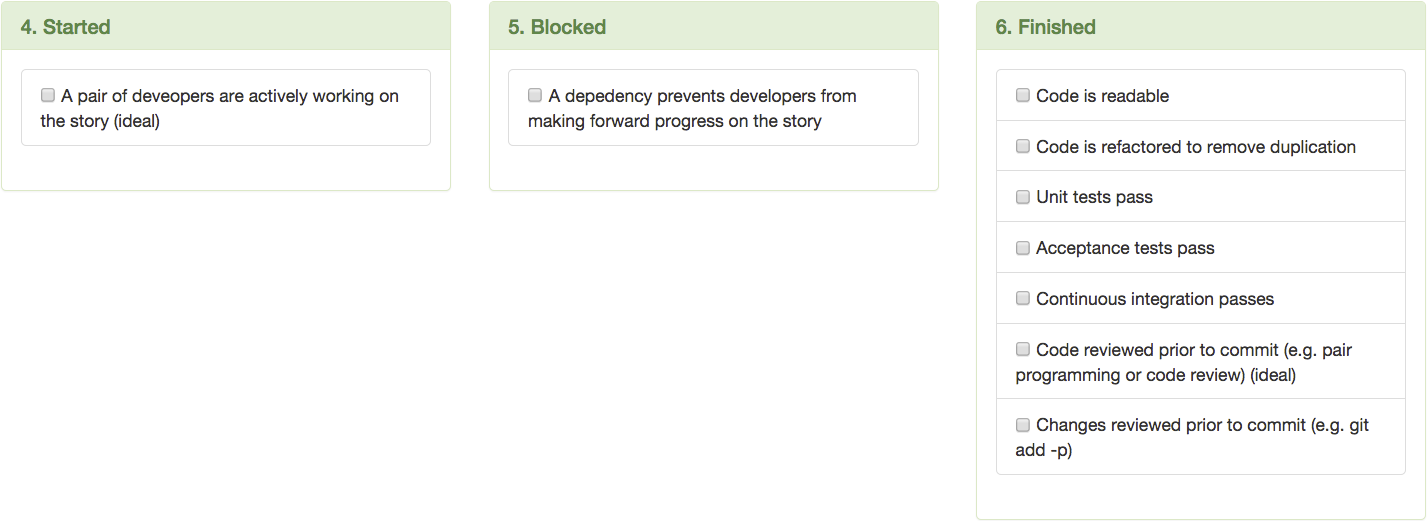
\includegraphics[width=6.25in]{pivotal_images/story_card2}
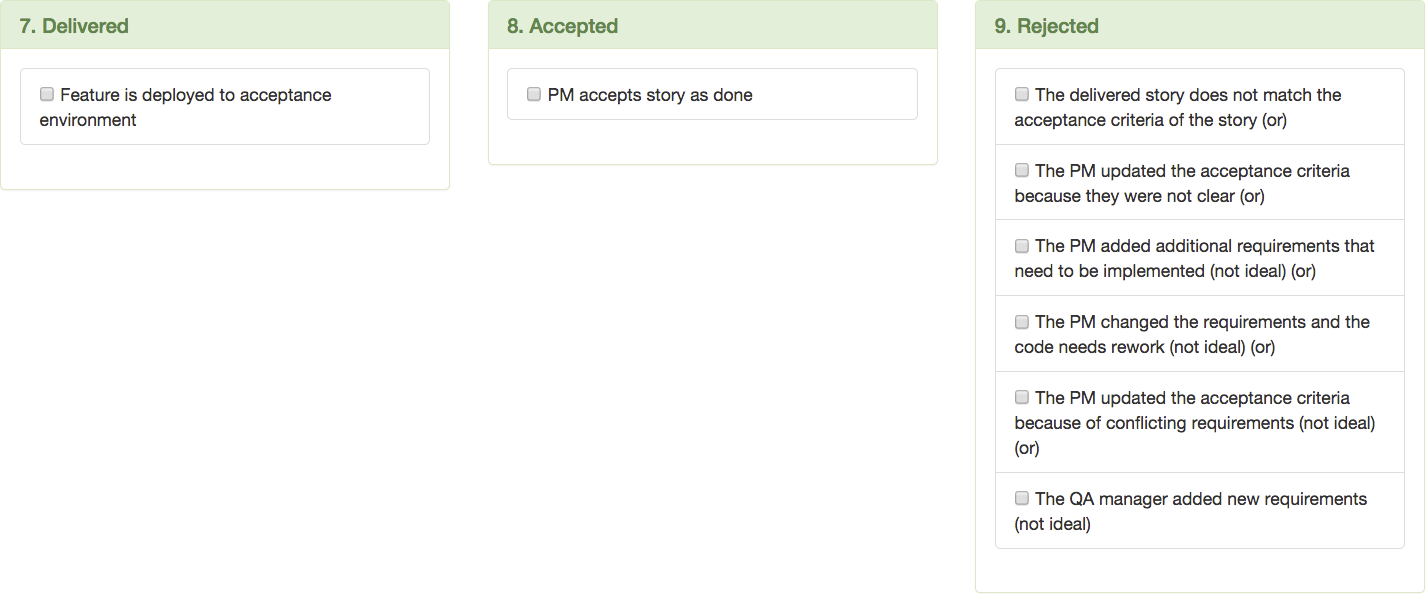
\includegraphics[width=6.25in]{pivotal_images/story_card3}
\caption{(Initial Results) Pivotal Kernel Extension for Story Card Alpha}
\label{KernelExtension}
\end{figure*}

\subsection{Discussion}
\label{Discussion}

Note: this section contains representative discussion about the current initial results. The purpose is to illustrate kind of discussion that could happen. Since the model is in flux, this section could change substantially.

\subsubsection{Evaluation of Results and Implications}

Figure \ref{KernelExtensionWorkflow} illustrates the state transitions of the \textbf{Story Card} alpha. Pivotal uses story cards in Pivotal Tracker to track and monitor the requirements for a system. The diagram identifies several problems with the kernel's fundamental structure of linear state machines. The normal flow from \textit{Named} to \textit{Accepted} is linear, however, story cards do revert to a previous state. During the Iteration Planning Meeting, stories categorized as \textit{Ready to be Pointed} can be delayed on pointing if the team realizes that the acceptance criteria is not clear or during the story's discussion, the product manager realizes that there are additional considerations that need to be addressed. \textit{Started} stories often become blocked on dependencies beyond the team's control. \textit{Started} stories sometimes get un-started due to changing project needs. Eventually \textit{Blocked} stories are un-blocked and transition to being ready to be worked on. Once stories are \textit{Delivered}, they can be \textit{Rejected} for a variety of 
reasons.

Figure \ref{KernelExtension} shows the checklists for each of these states. The checklists are typical of Essence kernels checklists with two exceptions. The checklists rely on both ``and" and  ``or" conditions to achieve a state. The data collection revealed the tension between prescriptive and descriptive modeling.

\subsubsection{Necessary modifications to the Essence structure}

The \textit{Rejected} state happens for a specific reason, thus achieving \textit{any} one of the checkpoint items causes the state to be achieved and the story to be \textit{Rejected}. The kernel would need a fundamental shift to support this since its underlying language requires accomplishing \textit{all} checklists. 

Two possible workarounds lose important details and are unappealing. Someone on the kernel author committee might suggest this situation be resolved by replacing the many checkpoints with a single ``the work is rejected" checkpoint. This path is unappealing as the proposed checkpoint both looses interesting information by dumbing-down the model, and simplifies the information into a trivial checkpoint that is redundant with the state's title. Another possible solution is to collapse the many checkpoints into a single statement that says ``A or B or C or D" as in ``the delivered story does not match the acceptance criteria of the story OR the PM updated ... or the PM added ... or the PM changed ... or the PM." This run-on sentence makes the checkpoint difficult to read and understand. 

There are typical and common reasons for a story to be rejected, two of which fit Pivotal's accepted flows for the work. 

\subsubsection{Descriptive versus Prescriptive}

In creating a kernel extension for Pivotal for iterative software projects, I've uncovered a tension between describing ``what is" versus ``the way it should be." It may be the case that this tension mirrors theories that are ``descriptive" versus those that are ``prescriptive." 

Some people do want a prescriptive model when I'm trying to create a descriptive one. After creating what really happens on a project, when I showed a draft extension to a co-worker, the engineer objected with parts of it. We have a shared understanding of how the work should be done, but in practice unusual circumstances occur that require us to respond accordingly. In practice, the product manager did reject delivered stories but not for reasons we would accept as part of our agreed-upon workflow. (Instead of creating a new story to capture new requirements. The product manager rejected a delivered story and added new functionality because rejecting was easier than writing a new story.) Just because something happens on a project does not mean that it should be part of the ``pivotal way" of doing things. As a researcher this presents a dilemma, am I documenting the way things really are, or the ``pivotal way."  It became apparent that I needed to separate out the descriptive from the  prescriptive. To solve this tension, I mark these distinctions on the model. 

I am biased in believing that software engineering research should start by observing what happens day-to-day on real software projects. As a benefit, any derived research is grounded by real empirical data. At the minimum, it provides a description of ``what is" and can form a Descriptive (Type I Analysis) theory. For example, understanding ``why software developers do not use static analysis tools" \cite{Johnson2013} could allow tool creators to better address those problems in their product. The Essence kernel does not do this. 

Instead, the Essence kernel is a prescriptive theory in that it accounts for how to run software by being opinionated in which goals a project should achieve (by including those checkpoint items) and which goals a project should not achieve (by excluding those checkpoint items.)

By crossing the line between describing what actually happens on a project into what should happen on a project, the Essence kernel runs the risk of both being wrong and not being useful.  It would be better to document typical ways people loose weight than to create a weight-loss program without empirical evidence. 

My intuition says that these ``prescriptive" or ``design and action" theories would need to be grounded in data too. Have you seen anything that talks about this?

I opened up the book, Guide to Advanced Empirical Software Engineering,  which sites Gregor (2006) to refresh myself on the types of theories.

Many of the differences between the prescribed and described kernel extensions can be explained by optional fields or optional interactions in Pivotal Tracker.

\subsubsection{Concerns?}
The proposed kernel extension resembles the story states in Pivotal Tracker. At first this was not intentional, but frequent tracking of the progress of the story from start to deployment lead to significant similarities between the kernel extension and the Pivotal Tracker story card states. At one point, this concerned me, perhaps Pivotal Tracker had too much undue influence on the kernel extension, however, since Pivotal built Pivotal Tracker to reflect the company's way of working, it should not be a surprise that the kernel extension has similar properties. 

\subsection{Threats to Validity}

External Validity. Generalizability across situations: The work done here analyzed software projects at the Silicon Valley office of Pivotal following Extreme Programming. The extension might not be applicable to other teams in industry following Extreme Programming. Replicating the results with other teams would mitigate this threat. Also, the teams following other iterative software development teams may or may not find value. Replicating this with teams following Scrum would mitigate this threat.

Internal Validity. Researcher bias: by using the participant-observer technique its possible that the researcher lost perspective and became biased by being a member of the team. An outside observer might see something the researcher missed. I used interviews and explicit reviews of the kernel to help mitigate this risk.



\section{Conclusion}
\label{Conclusions}

\subsection{Summary}
The original Essence kernel is method agnostic and does not directly support iterative development. During Essence Reflection meetings, student teams using the Essence kernel found value during project inception and start-up and found less value during an iterative construction phase. Since most of agile software development occurs via interactive construction adapting Essence kernel would increase its value to software development teams.

\subsection{Expected Impact}
A kernel extension for iterative software development would enable teams to find value from Essence during construction phases of a project.


\appendix
\section{Research Timeline}
\label{appendix}

\begin{table}[h]
\caption{Research Timeline}
\label{ResearchTimeline}
\centering
\begin{tabular}{|l|l|}
\hline
Semester    & Activities and Results  \\ \hline
Spring 2013 & Research: Facilitated Essence Reflection meetings and collected data for 4 master of software engineering teams. \\ \hline
Summer 2013 & Research: Facilitated Essence Reflection meetings and collected data for 3 master of software engineering teams.  \\ \hline
Fall 2013   & Research: Facilitated Essence Reflection meetings and collected data for 11 master of software engineering teams.  \\ \hline
Spring 2014 & \begin{tabular}[c]{@{}l@{}}Research: Facilitated Essence Reflection meetings and collected data for 2 master of software engineering teams.\\ Phd: Passed the ECE PhD qualifier.\\ Paper: Essence Reflection Meetings: Field Study, EASE 2014.\end{tabular} \\ \hline
Summer 2014 & \begin{tabular}[c]{@{}l@{}}Research: Facilitated Essence Reflection meetings and collected data for 3 master of software engineering teams.\\ Paper: State-based Monitoring and Goal-driven Project Steering: Field Study of the SEMAT Essence Framework, ICSE 2014.\end{tabular} \\ \hline
Fall 2014   & Research: Collected data from Participant-Observation on two projects at Pivotal Labs.  \\ \hline
Spring 2015 & \begin{tabular}[c]{@{}l@{}}Research: Collected data from Participant-Observation on one project at Pivotal Labs.\\ Paper: Towards Generating Essence Kernels Using Genetic Algorithms, SCSE 2015.\\ Tutorial: Using Essence Reflection Meetings in Team-Based Project Courses, SCSE 2015.\end{tabular} \\ \hline
Summer 2015 & \begin{tabular}[c]{@{}l@{}}Research: Kernel extension for iterative software projects.\\ Workshop: Essence in Team-Based Project Courses, CSEE\&T 2015. \end{tabular} \\ \hline                     
\end{tabular}
\end{table}

%% References
%%
%% Following citation commands can be used in the body text:
%% Usage of \cite is as follows:
%%   \cite{key}         ==>>  [#]
%%   \cite[chap. 2]{key} ==>> [#, chap. 2]
%%

%% References with bibTeX database:

\bibliographystyle{elsarticle-num}
% \bibliographystyle{elsarticle-harv}
% \bibliographystyle{elsarticle-num-names}
% \bibliographystyle{model1a-num-names}
% \bibliographystyle{model1b-num-names}
% \bibliographystyle{model1c-num-names}
% \bibliographystyle{model1-num-names}
% \bibliographystyle{model2-names}
% \bibliographystyle{model3a-num-names}
% \bibliographystyle{model3-num-names}
% \bibliographystyle{model4-names}
% \bibliographystyle{model5-names}
% \bibliographystyle{model6-num-names}

\bibliography{bibliography}


\end{document}

%%
%% End of file `elsarticle-template-num.tex'.




% "The checkpoints of an alpha state are joined by AND. The state of an alpha is deemed to be the most advanced (favourable) state for which all checkpoints are true." (OMG standard)

% "The checkpoints of a work product level of detail are joined by OR. The level of detail of a work product is deemed to be the most detailed level for which at least one checkpoint is true." (OMG standard)

fullfilledSuccessorLevel: my_LevelOfDetail 􏰃 my_LevelOfDetail fullfilledSuccessorLevel (l) =
if (l.successor = 􏰌) {l}
else
let mc = {c | c 􏰆 s.successor.checkpoints 􏰊 not c.isFullfilled} in (if (mc = 􏰌) {fullfilledSuccessor(s.successor)} else {l})


derive_current_state: my_Alpha 􏰃 my_State
derive_current_state (a) =
lets={s|s 􏰆 a.states 􏰊 {ps|ps.successor=s}= 􏰌} in fullfilledSuccessorState(s)